\section{FPGA}
This section will present an overview of the various components that need to be developed throughout this project.
In particular, the components that are specific to this application will be discussed in more detail.
See figure \ref{fig:fpga} for a view of the components.

\begin{figure}[H]
	\centering
	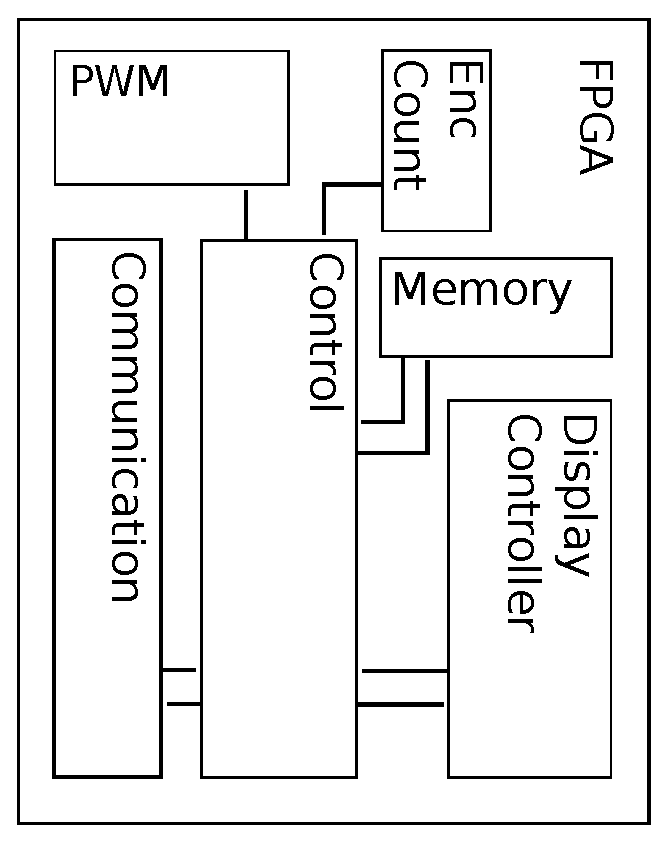
\includegraphics[angle=90,width=.5\linewidth]{images/fpga_block}
	\caption{An overview of the components to be written in VHDL.}
	\label{fig:fpga}
\end{figure}

\subsection{Communication}
This block will maintain the communication link with the PC.
As mentioned in previous sections, only one image is stored on the FPGA at any time.
This means that displaying a sequence of images has to be done by continuously rewriting the image present on the FPGA.
The communication will be done using $\mu$TosNet.
According to \cite{utosnet} $\mu$TosNet is capable of data rates of 10 Mbps.
Since each image is a known size of $40\times40\times12$ bits or 0.0192 Mbps, this would allow for transferring up to approximately 520 images per second.

\subsection{Enc. Count}
This block is responsible for calculating the current position of the motor.
It does this by monitoring the output of the photo sensor.
The photo sensor generates 16 pulses for each revolution of the motor.
This allows for a resolution of 22.5$^\circ$.
This is insufficient since an update is made every 2$^\circ$.
In order to artificially increase the resolution the time, $\Delta$t between each pulse is measured.
This makes it possible to estimate the time per degree by $t_d = \frac{\Delta\text{t}}{22.5^\circ}$.
Estimation of the angular position between pulses is then simply a matter of adding a degree to the position every $t_d$ seconds.
Both $t_d$ and the angular position are output from the block.

\subsection{PWM}
In order to keep the motor spinning at a constant velocity, it is necessary to continuously adjust the PWM used to control the motor.
Assuming a speed of 2200 RPM or $\approx$37 Hz as the goal, this results in $37\cdot360=13320$deg/sec.
This a a target $t_d$ of $\frac{1}{13320}=7.75\cdot10^{-5}$s.
The block will read the $t_d$ output from the enc. count block and adjust the PWM in order to minimize $|t_{d target}-t_d|$.

\subsection{Control}
This block is the connection point between all of the other blocks.
In an effort to simplify communication between blocks it was decided to create this block as a mediator.